\section{Results}

We train on 10000 simulated worlds with star objects of variable size placed at
random positions with random orientations. In each simulated world used for
training, we place only one object per world. We build our observation model
from simulated LIDAR scans from these worlds and the ground truth position and
orientation of the objects.

Then, we generate a LIDAR scan from an unseen simulated world with multiple
objects. This is shown in \figref{fig:sim_world}. We run our detector on this
LIDAR data. Because of the symmetry of the star, we test only orientations
between $\unit{0}{\degree}$ and $\unit{72}{\degree}$. The result of the detector
is shown in \figref{fig:detector}.

In \figref{fig:pr_curve}, we show the PR curve for the detections (after
non-maximal suppression) over 100 experiments with simulated world with 5
randomly placed objects each.
%
\begin{figure}
  \centering
  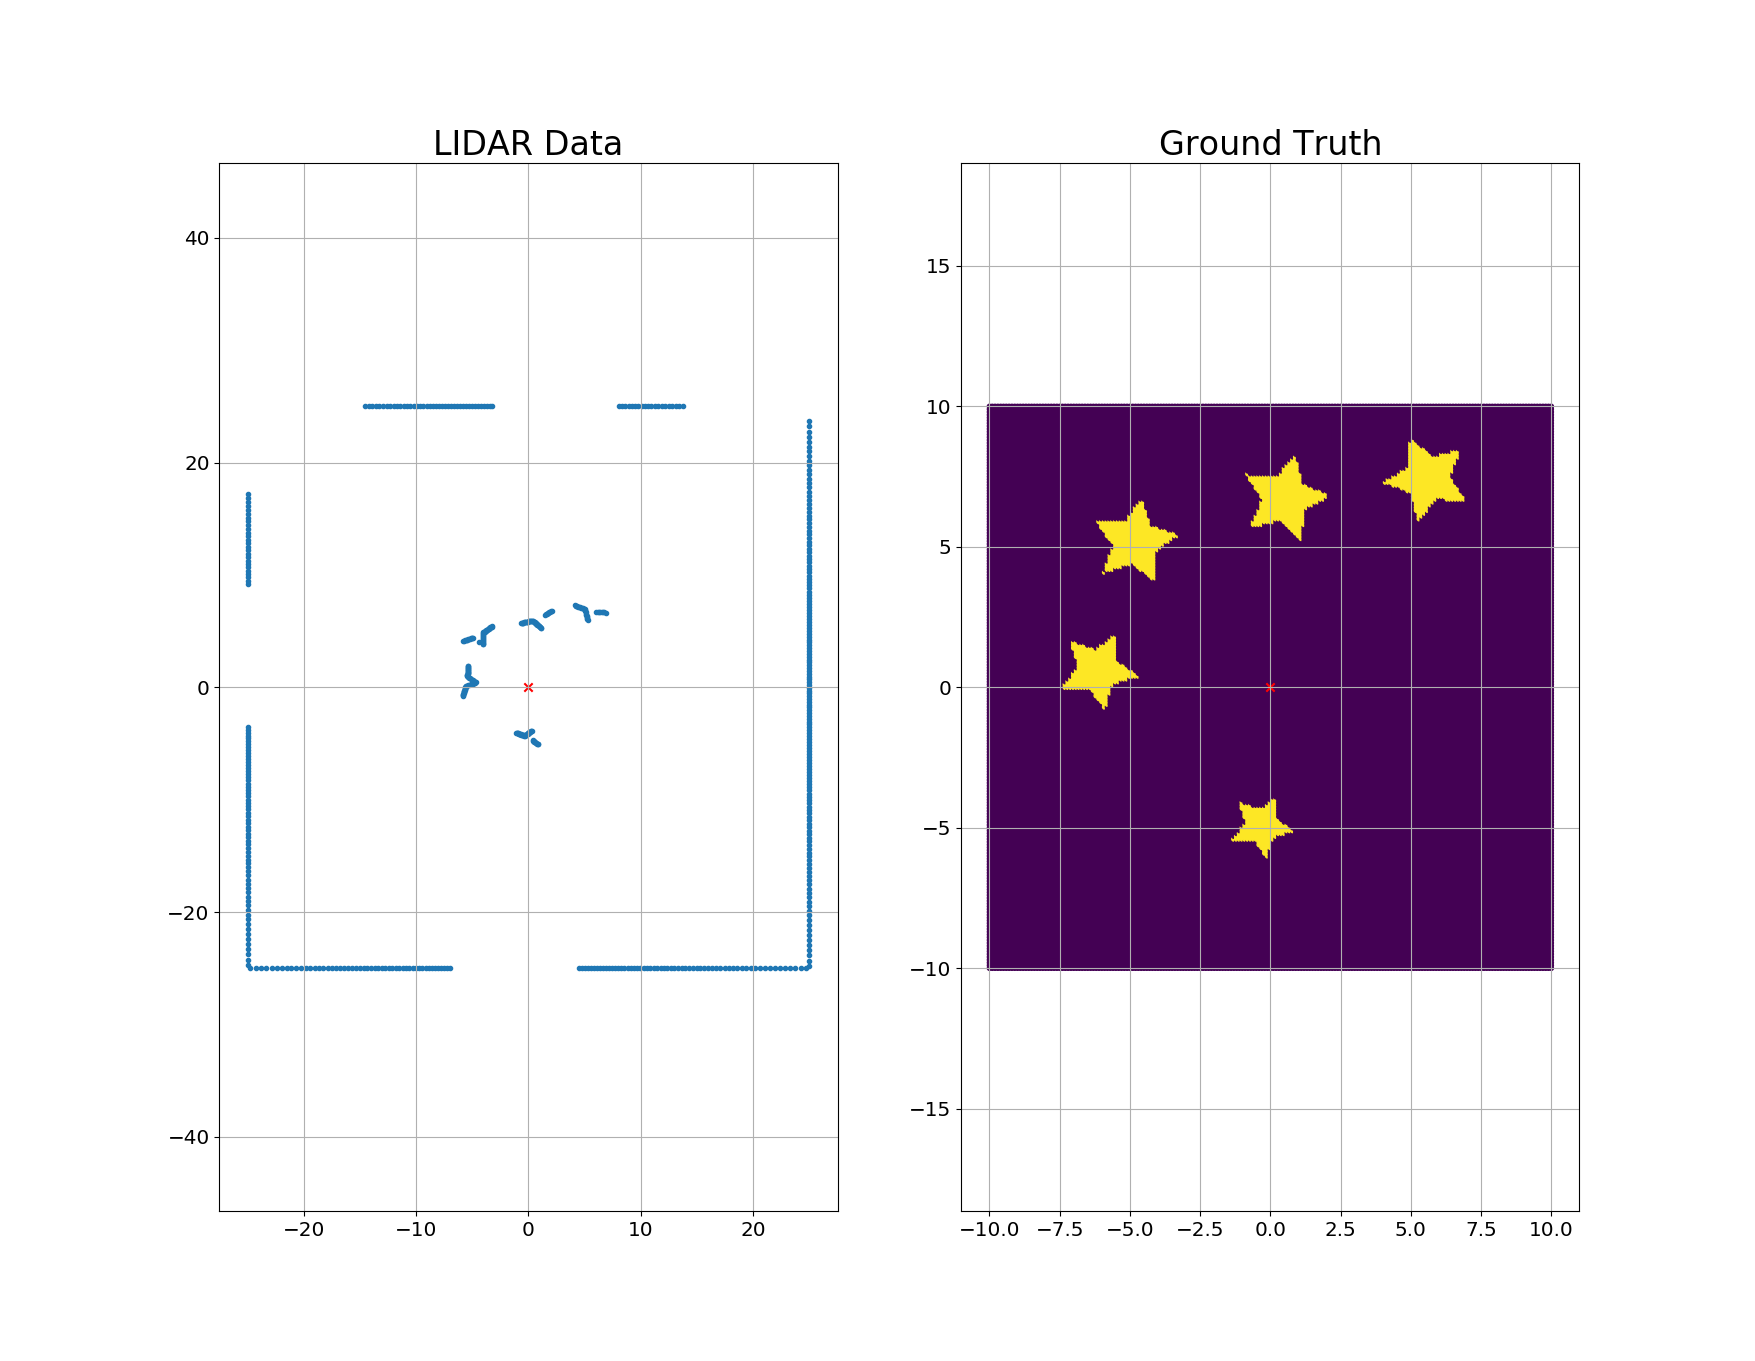
\includegraphics[width=\columnwidth]{figures/ground_truth.png}
  \caption{Simulation. On the left is the simular LIDAR scan of the environment.
    The right figure depicts the ground truth position of all objects in the
    scene.}
  \label{fig:sim_world}
\end{figure}
%
\begin{figure*}
  \centering
  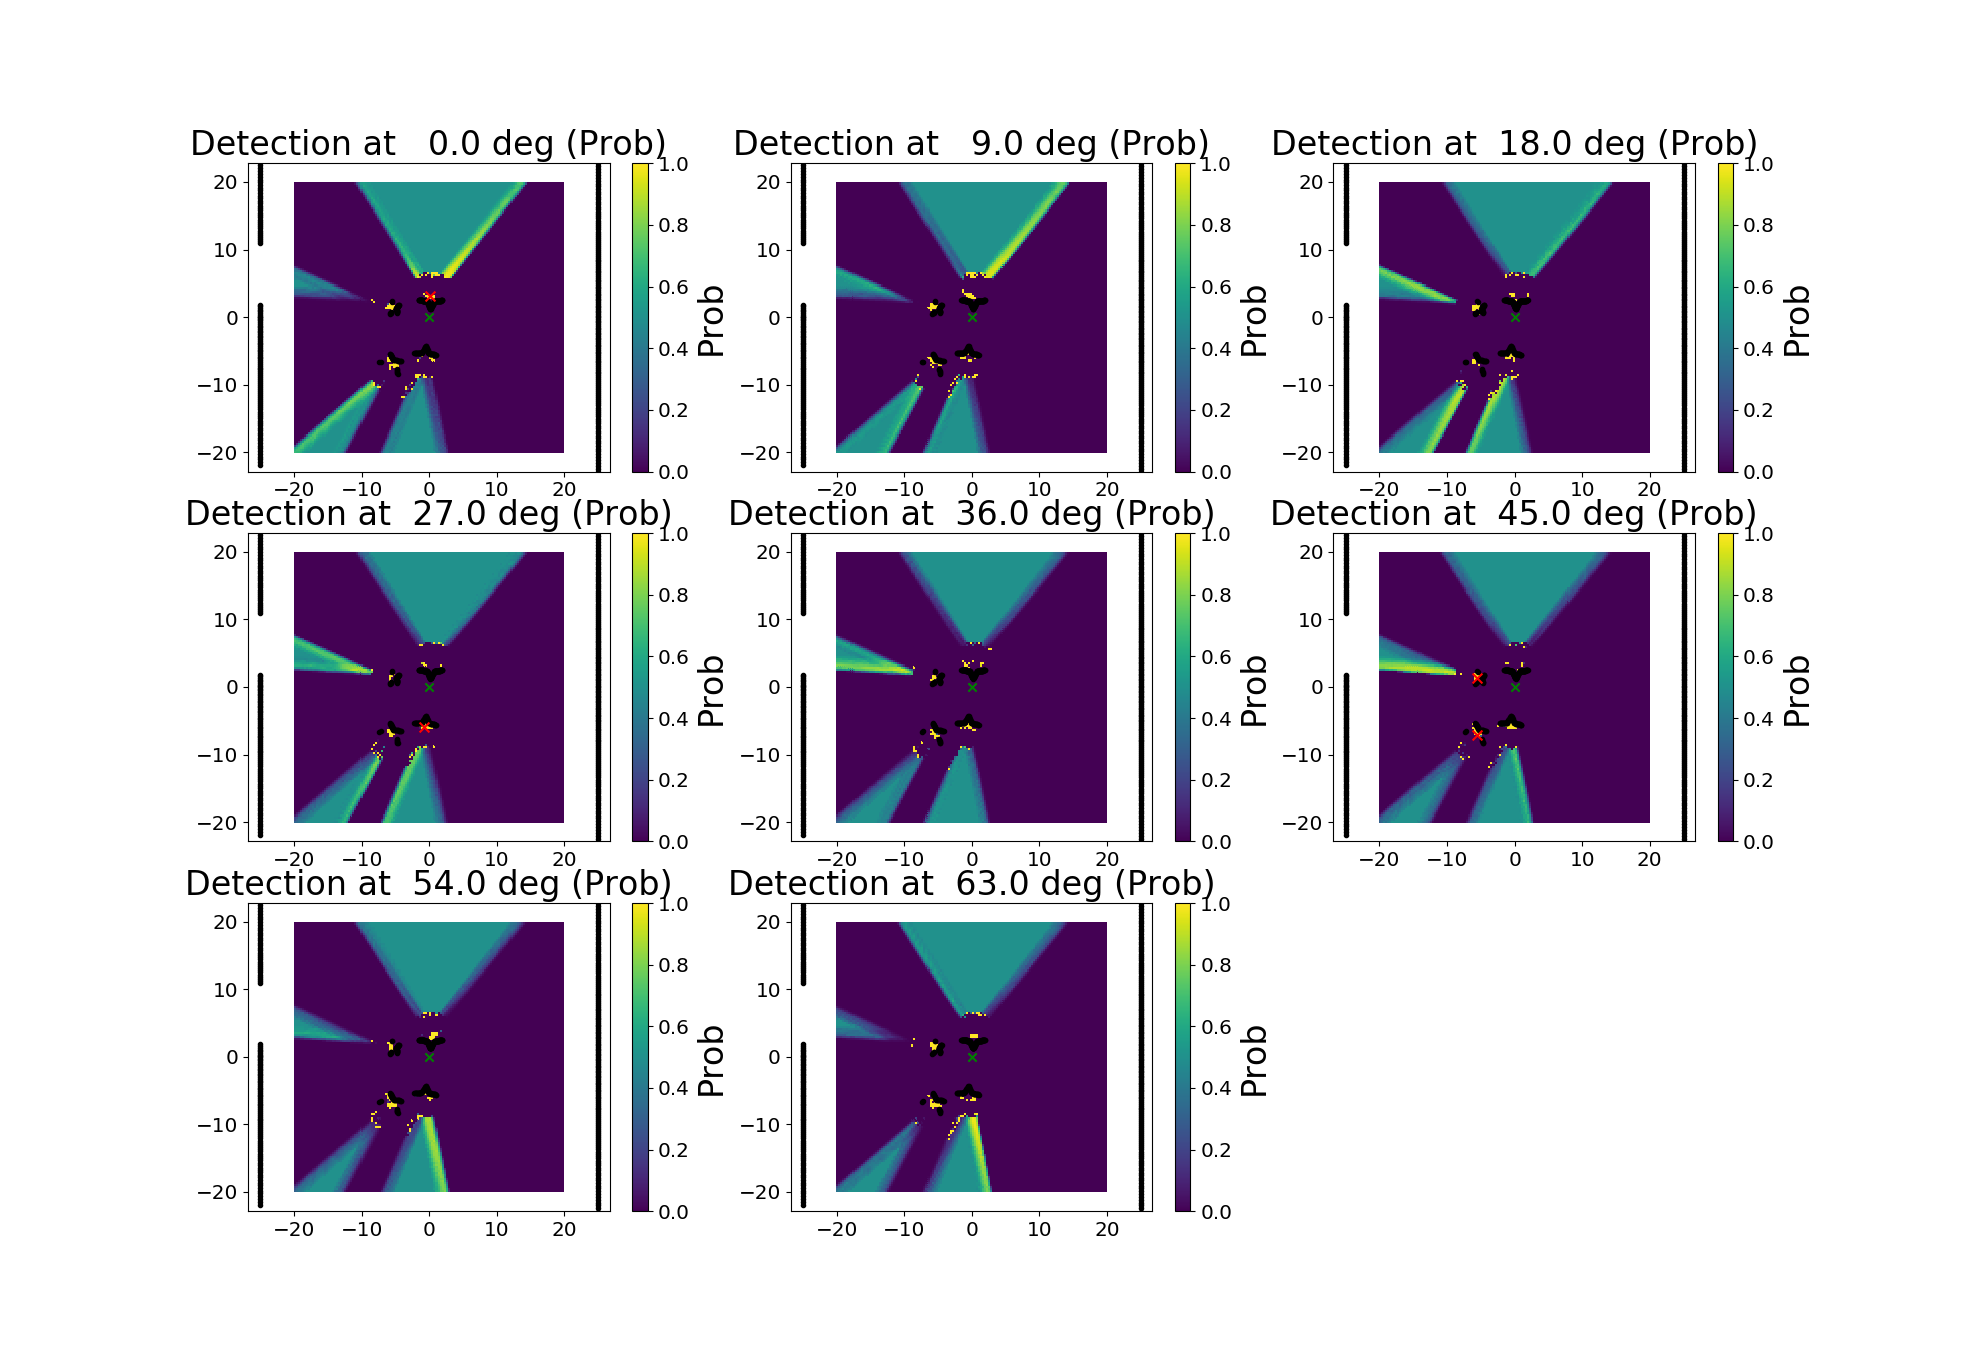
\includegraphics[width=\textwidth]{figures/detections.png}
  \caption{Result of detector. Non-maximal suppression results in detections
    marked with red x's}
  \label{fig:detector}
\end{figure*}
%
\begin{figure}
  \centering
  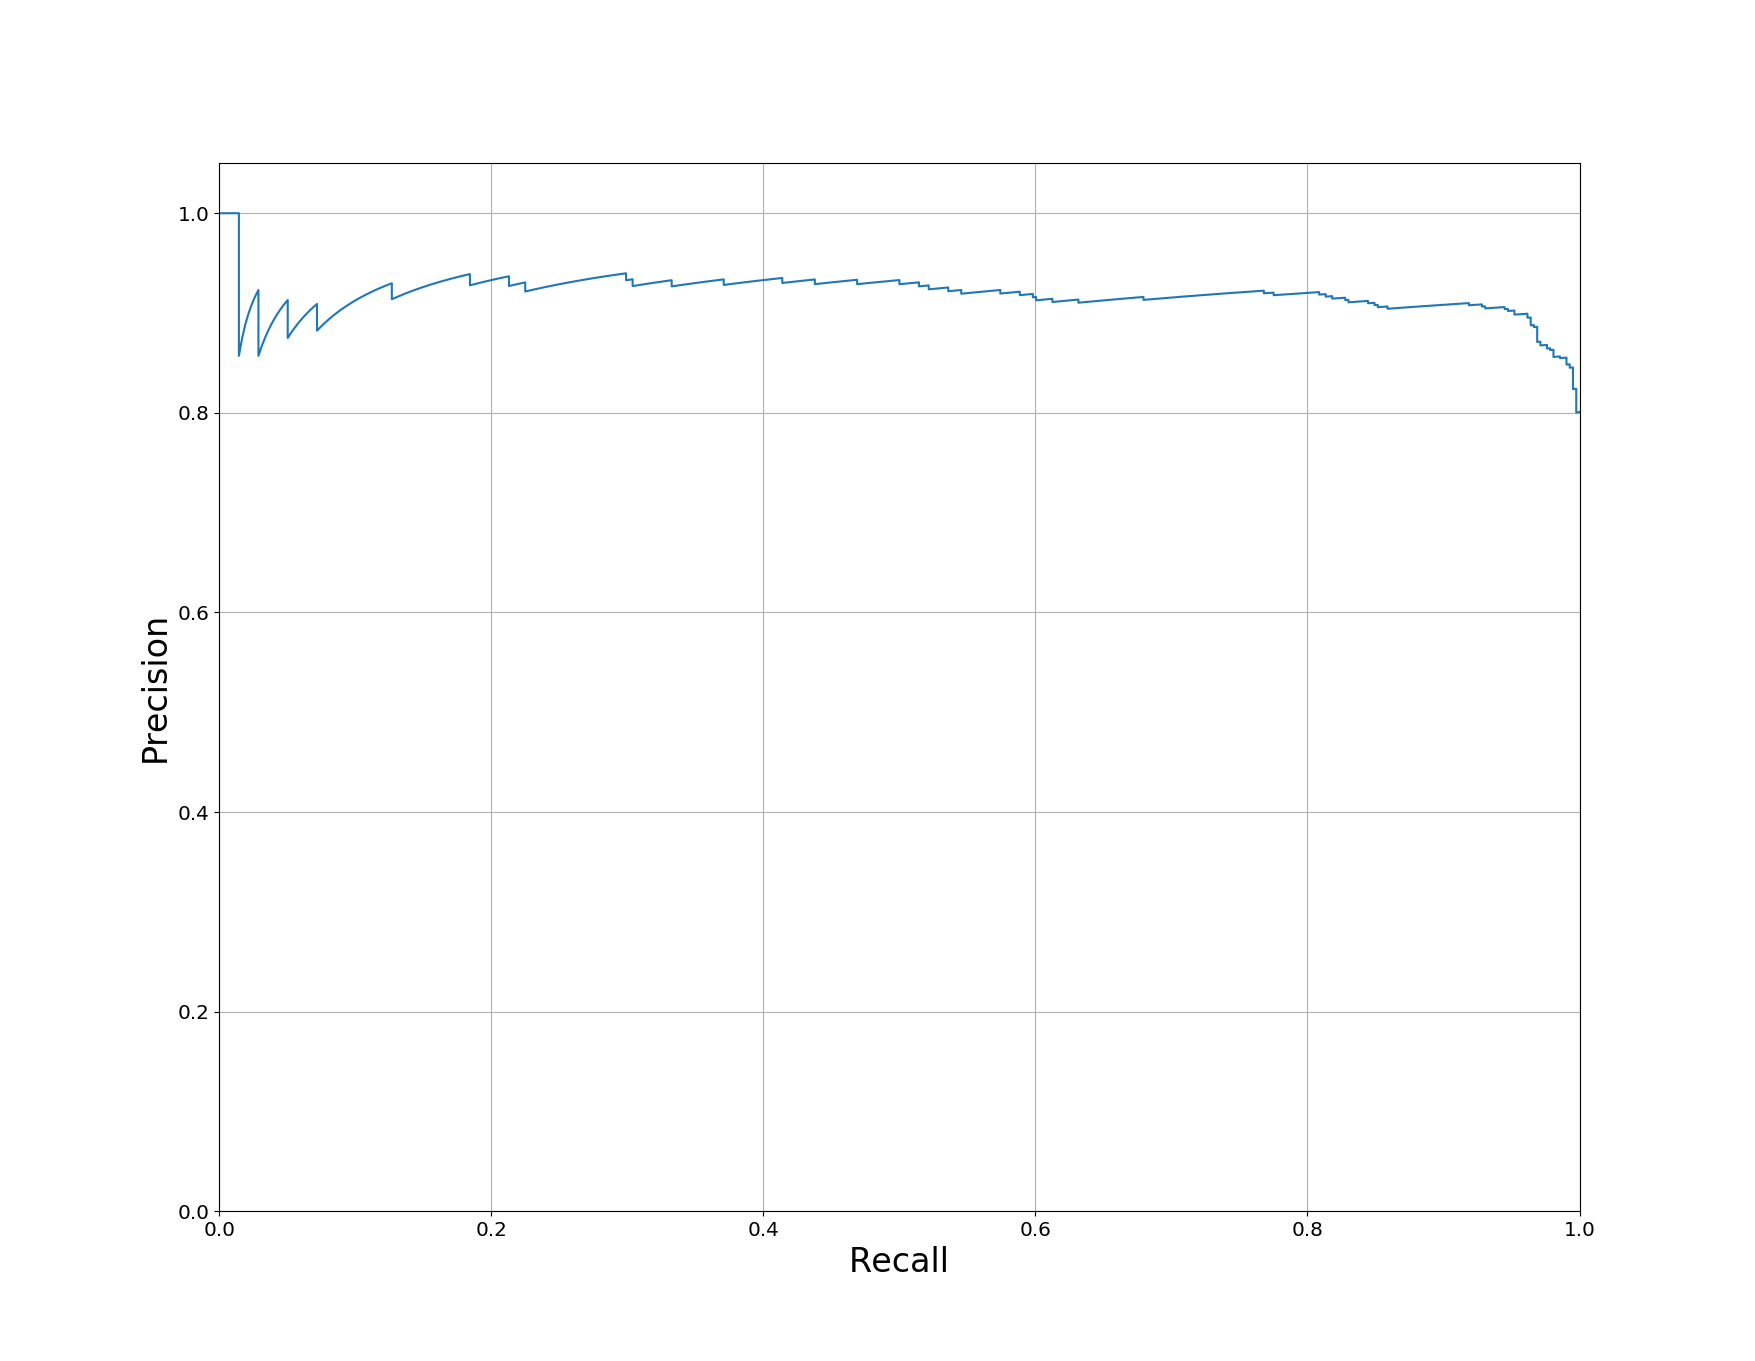
\includegraphics[width=\columnwidth]{figures/pr_curve.png}
  \caption{PR curve for detections}.
  \label{fig:pr_curve}
\end{figure}
